% !TeX root = ../../../main.tex
\subsubsection{Evaluation of Clinical Textual Time Series Quality}
\label{ch05:sec:evaluation-of-tts-quality}

Using the 200 manually annotated case reports as reference, we evaluated textual time series quality across LLM annotators and runs using event match recall, precision, and F1, temporal concordance (c-index), and AULTC. Table~\ref{ch05:tab:model_comparison} reports mean and standard deviation across runs for seven LLM variants: \texttt{Llama 3.3 70B}, \texttt{DeepSeek-R1}, \texttt{DeepSeek-V3}, \texttt{OpenAI GPT-5}, \texttt{OpenAI O4-mini}, \texttt{OpenAI O3}, and \texttt{OpenAI O1}.

\ChFiveRebuttal{
We additionally evaluated event match precision and F1 to account for model-generated events that were not matched to the manually annotated timeline (Tables~\ref{ch05:tab:model_comparison} and~\ref{ch05:tab:bootstrap_intervals}). Precision varied from 0.756 for GPT-5 to 0.873 for O1, while recall showed the opposite pattern for these models (0.845 for GPT-5 versus 0.637 for O1), illustrating differences in the precision--recall tradeoff across models. F1 ranged from 0.712 to 0.798. Bootstrap 95\% confidence intervals for precision and F1 are reported in Table~\ref{ch05:tab:bootstrap_intervals}. Table~\ref{ch05:tab:model_comparison_lapjv} also includes precision and F1 under the LAPJV-based matching analysis.
}



% !TeX root = ../../../main.tex
\begin{table}[htbp]
\caption{\ChFiveRebuttal{Comparison of models on Event Match Rate (Recall), Event Match Precision, Event Match F1, Concordance, and AULTC with respect to 200 manually annotated case reports across 5 independent runs for each model.}}\ChFiveFloatLabel{ch05:tab:model_comparison}
\ChFiveTableBodyStart
\begin{ChFiveFloatBody}


\footnotesize
\centering
\setlength{\tabcolsep}{3pt}


\begin{tabular}{lccccc}
\hline
\textbf{Model} &
\begin{tabular}{c}\textbf{Event Match}\\\textbf{ Recall}\end{tabular} &
\begin{tabular}{c}\textbf{Event Match}\\\textbf{Precision}\end{tabular} &
\begin{tabular}{c}\textbf{Event Match}\\\textbf{F1}\end{tabular} &
\textbf{Concordance} &
\textbf{AULTC} \\
\hline
\texttt{Llama 3.3 70B}
& 0.673 $\pm$ 0.003
& 0.757 $\pm$ 0.036
& 0.712 $\pm$ 0.015
& 0.846 $\pm$ 0.002
& 0.721 $\pm$ 0.001 \\

\texttt{DeepSeek-R1}
& 0.746 $\pm$ 0.008
& 0.788 $\pm$ 0.006
& 0.766 $\pm$ 0.005
& 0.773 $\pm$ 0.010
& 0.728 $\pm$ 0.004 \\

\texttt{DeepSeek-V3}
& 0.760 $\pm$ 0.004
& 0.796 $\pm$ 0.006
& 0.778 $\pm$ 0.004
& 0.783 $\pm$ 0.007
& 0.731 $\pm$ 0.002 \\

\texttt{OpenAI GPT-5}
& \textbf{0.845 $\pm$ 0.005}
& 0.756 $\pm$ 0.007
& \textbf{0.798 $\pm$ 0.003}
& \textbf{0.902 $\pm$ 0.002}
& 0.722 $\pm$ 0.001 \\

\texttt{OpenAI O4-mini}
& 0.748 $\pm$ 0.019
& 0.814 $\pm$ 0.015
& 0.779 $\pm$ 0.017
& 0.846 $\pm$ 0.006
& \textbf{0.750 $\pm$ 0.002} \\

\texttt{OpenAI O3}
& 0.733 $\pm$ 0.003
& 0.837 $\pm$ 0.003
& 0.782 $\pm$ 0.002
& 0.898 $\pm$ 0.002
& 0.737 $\pm$ 0.003 \\

\texttt{OpenAI O1}
& 0.637 $\pm$ 0.007
& \textbf{0.873 $\pm$ 0.003}
& 0.737 $\pm$ 0.005
& 0.885 $\pm$ 0.002
& 0.732 $\pm$ 0.002 \\
\hline
\end{tabular}


\end{ChFiveFloatBody}
\end{table}




% !TeX root = ../../../main.tex
\begin{table}[htbp]
\caption{\ChFiveRebuttal{Bootstrap 95\% confidence intervals for Event Match Rate (Recall), Event Match Precision, Event Match F1, Concordance, and AULTC across models evaluated on the 200 manually annotated case reports.}}\ChFiveFloatLabel{ch05:tab:bootstrap_intervals}
\ChFiveTableBodyStart
\begin{ChFiveFloatBody}


\footnotesize
\centering
\setlength{\tabcolsep}{3pt}


\begin{tabular}{lccccc}
\hline
\textbf{Model} &
\begin{tabular}{c}\textbf{Event Match}\\\textbf{Recall}\end{tabular} &
\begin{tabular}{c}\textbf{Event Match}\\\textbf{Precision}\end{tabular} &
\begin{tabular}{c}\textbf{Event Match}\\\textbf{F1}\end{tabular} &
\textbf{Concordance} &
\textbf{AULTC} \\
&
\textbf{(95\% CI)} &
\textbf{(95\% CI)} &
\textbf{(95\% CI)} &
\textbf{(95\% CI)} &
\textbf{(95\% CI)} \\
\hline
\texttt{Llama 3.3 70B}
& [0.647, 0.715]
& [0.564, 0.835]
& [0.603, 0.770]
& [0.819, 0.864]
& [0.698, 0.746] \\

\texttt{DeepSeek-R1}
& [0.702, 0.771]
& [0.760, 0.807]
& [0.730, 0.789]
& [0.747, 0.782]
& [0.707, 0.751] \\

\texttt{DeepSeek-V3}
& [0.736, 0.795]
& [0.782, 0.825]
& [0.758, 0.810]
& [0.756, 0.813]
& [0.708, 0.753] \\

\texttt{OpenAI GPT-5}
& [0.812, 0.866]
& [0.751, 0.792]
& [0.780, 0.827]
& [0.889, 0.911]
& [0.702, 0.745] \\

\texttt{OpenAI O4-mini}
& [0.695, 0.764]
& [0.772, 0.828]
& [0.732, 0.795]
& [0.824, 0.868]
& [0.727, 0.772] \\

\texttt{OpenAI O3}
& [0.703, 0.765]
& [0.818, 0.855]
& [0.756, 0.808]
& [0.880, 0.915]
& [0.721, 0.761] \\

\texttt{OpenAI O1}
& [0.612, 0.686]
& [0.864, 0.890]
& [0.717, 0.775]
& [0.869, 0.900]
& [0.712, 0.753] \\
\hline
\end{tabular}


\end{ChFiveFloatBody}
\end{table}



To quantify uncertainty from a complementary perspective, we also performed a bootstrap analysis based on resampling the 200 annotated cases with replacement and recomputing metrics to obtain 95\% confidence intervals. These intervals characterize variability arising from the composition of the reference set, whereas the across-run standard deviations reflect variability in model sampling. The full set of bootstrap intervals is reported in Table~\ref{ch05:tab:bootstrap_intervals}.

% \begin{figure}[!tbp]
% \centering
%     \begin{minipage}[t]{0.242\textwidth}
%     \centering
%     \includegraphics[page=1, width=\linewidth]{Plots_tables/pmoa_updated_man_figs.pdf}
%     \end{minipage}
%     \hfill
%     \begin{minipage}[t]{0.242\textwidth}
%     \centering
%     \includegraphics[page=2, width=\linewidth]{Plots_tables/pmoa_updated_man_figs.pdf}
%     \end{minipage}
%     \hfill
%     \begin{minipage}[t]{0.242\textwidth}
%     \centering
%     \includegraphics[page=3, width=\linewidth]{Plots_tables/pmoa_updated_man_figs.pdf}
%     \end{minipage}
%     \hfill
%     \begin{minipage}[t]{0.242\textwidth}
%     \centering
%     \includegraphics[page=4, width=\linewidth]{Plots_tables/pmoa_updated_man_figs.pdf}
%     \end{minipage}
%     \caption{Comparison of different LLM for extracting temporal clinical events from case reports. From left to right: (\textbf{A}) event match cumulative distribution function, (\textbf{B}) concordance box plots, (\textbf{C}) time discrepancy from manual annotation timestamps among matched events (overall), and (\textbf{D}) time discrepancy disaggregated by clinician annotator timestamp (time from presentation). 
%     %\textcolor{red}{Have same figure for LAPJV?}
%     }
%     \label{fig:tts_evaluation}
%     \vspace{-10pt}
% \end{figure}




% !TeX root = ../../../main.tex
\begin{figure}[htbp]
\begin{ChFiveFloatBody}

\centering

% First row: panels A and B
\begin{minipage}[t]{0.49\linewidth}
    \centering
    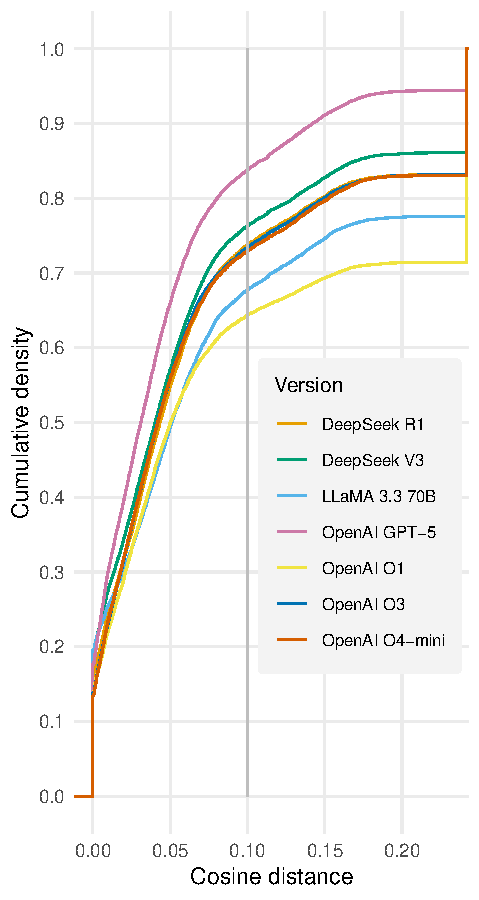
\includegraphics[
        page=1,
        width=0.8\linewidth
    ]{Chapters/chapter-05/images/Plots_tables/pmoa_updated_man_figs.pdf}
\end{minipage}
\hfill
\begin{minipage}[t]{0.49\linewidth}
    \centering
    \includegraphics[
        page=2,
        width=0.8\linewidth
    ]{Chapters/chapter-05/images/Plots_tables/pmoa_updated_man_figs.pdf}
\end{minipage}

\par\medskip

% Second row: panels C and D
\begin{minipage}[t]{0.49\linewidth}
    \centering
    \includegraphics[
        page=3,
        width=0.8\linewidth
    ]{Chapters/chapter-05/images/Plots_tables/pmoa_updated_man_figs.pdf}
\end{minipage}
\hfill
\begin{minipage}[t]{0.49\linewidth}
    \centering
    \includegraphics[
        page=4,
        width=0.8\linewidth
    ]{Chapters/chapter-05/images/Plots_tables/pmoa_updated_man_figs.pdf}
\end{minipage}





\end{ChFiveFloatBody}
\caption{
Comparison of different LLMs for extracting temporal clinical events
from case reports:
(\textbf{A}) cumulative distribution of event-matching cosine distances;
(\textbf{B}) temporal-concordance box plots;
(\textbf{C}) timestamp discrepancies between model-generated and manual
annotations among semantically matched events; and
(\textbf{D}) timestamp discrepancies stratified by the clinician-annotated
time relative to presentation.
}\ChFiveFloatLabel{ch05:fig:tts_evaluation}
\end{figure}



\paragraph{Text Event Match Performance}
\label{ch05:sec:text-event-match-performance}
Figure~\ref{ch05:fig:tts_evaluation} (A) shows the cumulative distributions of cosine distances between model-generated and reference event descriptions, with a threshold of 0.1 used to define a successful semantic match. At this threshold, 
\ChFiveRebuttal{
\texttt{GPT-5} had the highest mean event-recall point estimate (0.845), followed by \texttt{DeepSeek-V3} (0.760), \texttt{O4-mini} (0.748), and \texttt{DeepSeek-R1} (0.746). \texttt{O3} and \texttt{Llama 3.3 70B} had mean recall values of 0.733 and 0.673, respectively, while \texttt{O1} had the lowest mean recall (0.637). These point estimates show variation across models in the proportion of manually annotated clinical events recovered under the selected semantic-matching threshold.
}
% \ChFiveRebuttal{
% \texttt{GPT-5} achieved the highest mean event recall (0.845), followed by \texttt{DeepSeek-V3} (0.760), \texttt{O4-mini} (0.748), and \texttt{DeepSeek-R1} (0.746). \texttt{O3} and \texttt{Llama 3.3 70B} achieved lower recall of 0.733 and 0.673, respectively, while \texttt{O1} had the lowest recall (0.637). These results indicate meaningful differences across models in the proportion of manually annotated clinical events recovered under the selected semantic-matching threshold.
% }

\paragraph{Temporal Ordering Performance}
\label{ch05:sec:temporal-ordering-performance}

Using the same similarity threshold to identify matched events, temporal ordering accuracy was evaluated with the concordance index (c-index). As shown in Figure~\ref{ch05:fig:tts_evaluation} (B),
\ChFiveRebuttal{
\texttt{GPT-5} had the highest mean concordance point estimate (0.902), followed closely by \texttt{O3} (0.898) and \texttt{O1} (0.885). \texttt{Llama 3.3 70B} and \texttt{O4-mini} both had mean concordance of 0.846, while \texttt{DeepSeek-V3} and \texttt{DeepSeek-R1} had mean concordance of 0.783 and 0.773, respectively. However, the bootstrap 95\% confidence intervals for the leading models overlapped. We therefore interpret the ordering of the mean estimates descriptively and do not consider these results evidence that one model was statistically superior in temporal ordering.
The differences between event recall and concordance across models illustrate that these metrics capture distinct aspects of timeline quality. For example, \texttt{O1} had the lowest event recall but relatively high concordance among the events that were successfully matched.
}
% \ChFiveRebuttal{\texttt{GPT-5} achieved the highest mean concordance (0.902), closely followed by \texttt{O3} (0.898) and \texttt{O1} (0.885). \texttt{Llama 3.3 70B} and \texttt{O4-mini} both achieved concordance of 0.846, while \texttt{DeepSeek-V3} and \texttt{DeepSeek-R1} had lower concordance of 0.783 and 0.773, respectively. The differences between event recall and concordance across models illustrate that event recovery and temporal ordering capture distinct aspects of timeline quality. For example, \texttt{O1} had the lowest event recall but relatively high concordance among the events that were successfully matched.}
This contrast highlights that models that align fewer but clearer events may achieve high ordering scores, whereas models with broader coverage face a more challenging ordering task.


\paragraph{Time Discrepancy Analysis}
\label{ch05:sec:time-descrepancy-analysis}
Figure~\ref{ch05:fig:tts_evaluation} (C, D) presents cumulative distributions of log-scaled time discrepancies between predicted and reference timestamps for semantically matched events. 
\ChFiveRebuttal{
\texttt{O4-mini} had the highest mean AULTC point estimate (0.750), followed by \texttt{O3} (0.737). \texttt{O1}, \texttt{DeepSeek-V3}, and \texttt{DeepSeek-R1} had similar intermediate mean values of 0.732, 0.731, and 0.728, respectively, while \texttt{GPT-5} (0.722) and \texttt{Llama 3.3 70B} (0.721) had the lowest mean AULTC values. However, the bootstrap 95\% confidence intervals overlapped across several models. We therefore treat this ordering as descriptive and do not interpret the higher mean for \texttt{O4-mini} as evidence of statistically distinct superiority in timestamp accuracy.
The variation in mean AULTC was smaller than the variation observed for event recall and temporal concordance. The interval-stratified analysis in Figure~\ref{ch05:fig:tts_evaluation} (D) further shows how timestamp accuracy varies with temporal distance from the admission reference time.
}
% \ChFiveRebuttal{
% \texttt{O4-mini} achieved the highest mean AULTC (0.750), followed by \texttt{O3} (0.737). \texttt{O1}, \texttt{DeepSeek-V3}, and \texttt{DeepSeek-R1} achieved similar intermediate values of 0.732, 0.731, and 0.728, respectively, while \texttt{GPT-5} (0.722) and \texttt{Llama 3.3 70B} (0.721) had the lowest mean AULTC values. 
% Notably, the spread in AULTC performance is less pronounced than that observed for the event match rate and concordance.
% The interval-stratified analysis in Figure~\ref{ch05:fig:tts_evaluation} (D) further shows how timestamp accuracy varies with temporal distance from the admission reference time.
% }

Taken together, these results show that semantic matching, temporal ordering, and timestamp accuracy provide complementary views of textual time series quality. Because the leading mean estimates differ across metrics and their bootstrap confidence intervals frequently overlap, we do not designate a single best-performing model.

\paragraph{Timestamp Provenance Audit}
\label{ch05:sec:timestamp-provenance-audit}

\ChFiveRebuttal{
The production TTS schema stores a single timestamp for each extracted event and does not distinguish whether the timestamp is directly supported by temporal information in the source text or inferred from narrative context. Because this provenance was not retained during full-corpus generation, we conducted a targeted audit of the 200 evaluation reports using GPT-5. We retained the original event-time extraction task while adding a binary \emph{known} indicator for each event. \emph{known=1} was assigned when the timestamp was anchored by admission/presentation or directly supported by an absolute or relative temporal expression in the source text; \emph{known=0} was assigned when the timestamp was inferred from narrative context or clinical judgment.
}

\ChFiveRebuttal{
Across 11,618 extracted events, 6,314 (54.35\%) timestamps were text-supported or directly anchored (\emph{known=1}), while 5,304 (45.65\%) were inferred (\emph{known=0}). At the case level, the median proportion of text-supported timestamps was 53.29\% (IQR: 31.58\%--75.52\%). Thus, while a slight majority of timestamps could be tied directly to temporal evidence under this definition, temporal imputation accounts for a considerable fraction of the generated timelines. This audit is limited to GPT-5 outputs on the evaluation sample and does not provide provenance annotations for the full corpus or establish that the observed proportions generalize to other extraction models.
}

\paragraph{Inter-annotator agreement on a GLP1-RA subset}
\label{ch05:glp_iaa}

\ChFiveRebuttal{To contextualize agreement with the single-expert reference set, we also analyzed a separate 140-case report subset of PMOA-TTS involving patients who took GLP-1 RA (Glucagon-like Peptide Receptor Agonists) medications. Two clinically trained annotators independently constructed event-time timelines for this subset using the same annotation framework. Using Annotator 1 as the reference and the same matching and temporal metrics used for the model evaluation, Annotator 2 achieved an event match rate of 0.811, temporal concordance of 0.798, and AULTC of 0.702.}

